Lancer une partie pour jouer un morceau au piano et gagner le plus de points possible!
\\\\
Pour lancer une partie, sélectionnez d’abord une chanson depuis votre page personnelle, ou parmis les résultats d’une recherche (cf. section suivante).

\begin{figure}[H]
	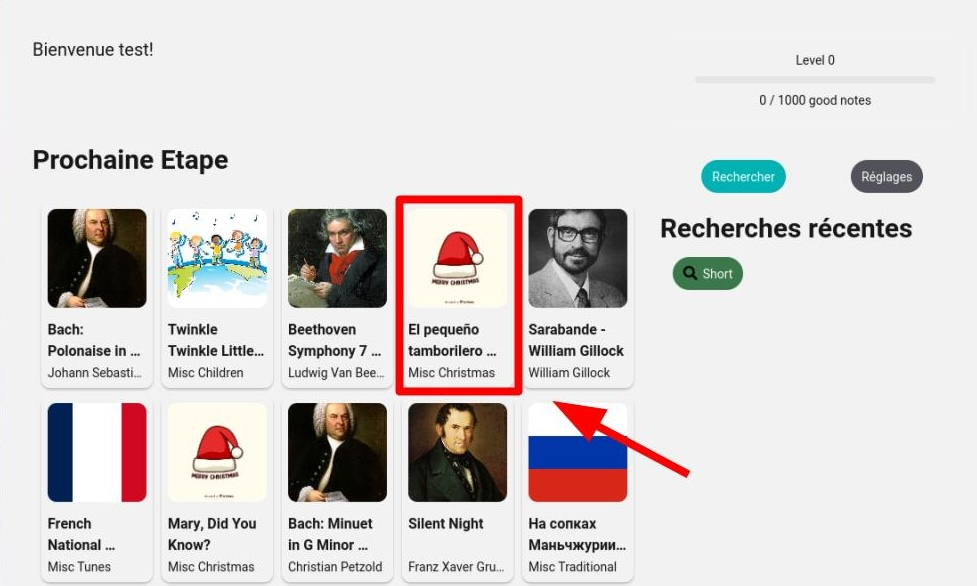
\includegraphics[width=\linewidth]{../\dir/guide/play/home.jpg}
	\caption{Acceder à une chanson depuis la page d'accueil}
\end{figure}

\begin{figure}[H]
	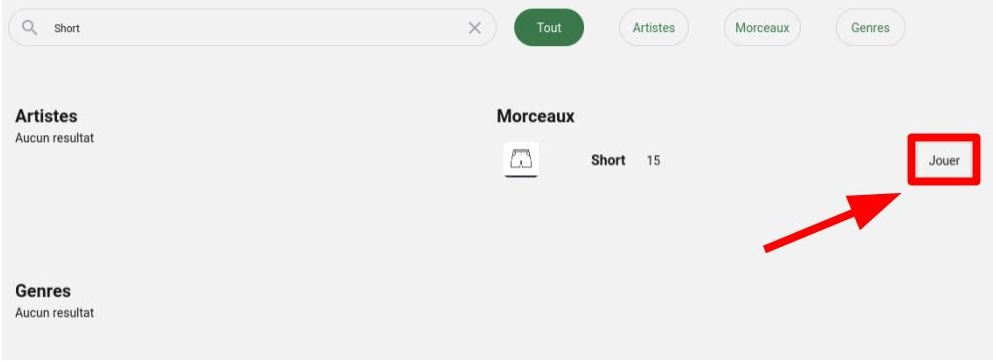
\includegraphics[width=\linewidth]{../\dir/guide/play/search.jpg}
	\caption{Acceder à une chanson depuis la page de recherche}
\end{figure}

Vous arriverez sur une page de lobby, vous présentant succinctement la chanson.
Avant de lancer la partie, assurez-vous que votre piano MIDI soit connecté.
Cliquez sur le bouton Jouer.

\begin{figure}[H]
	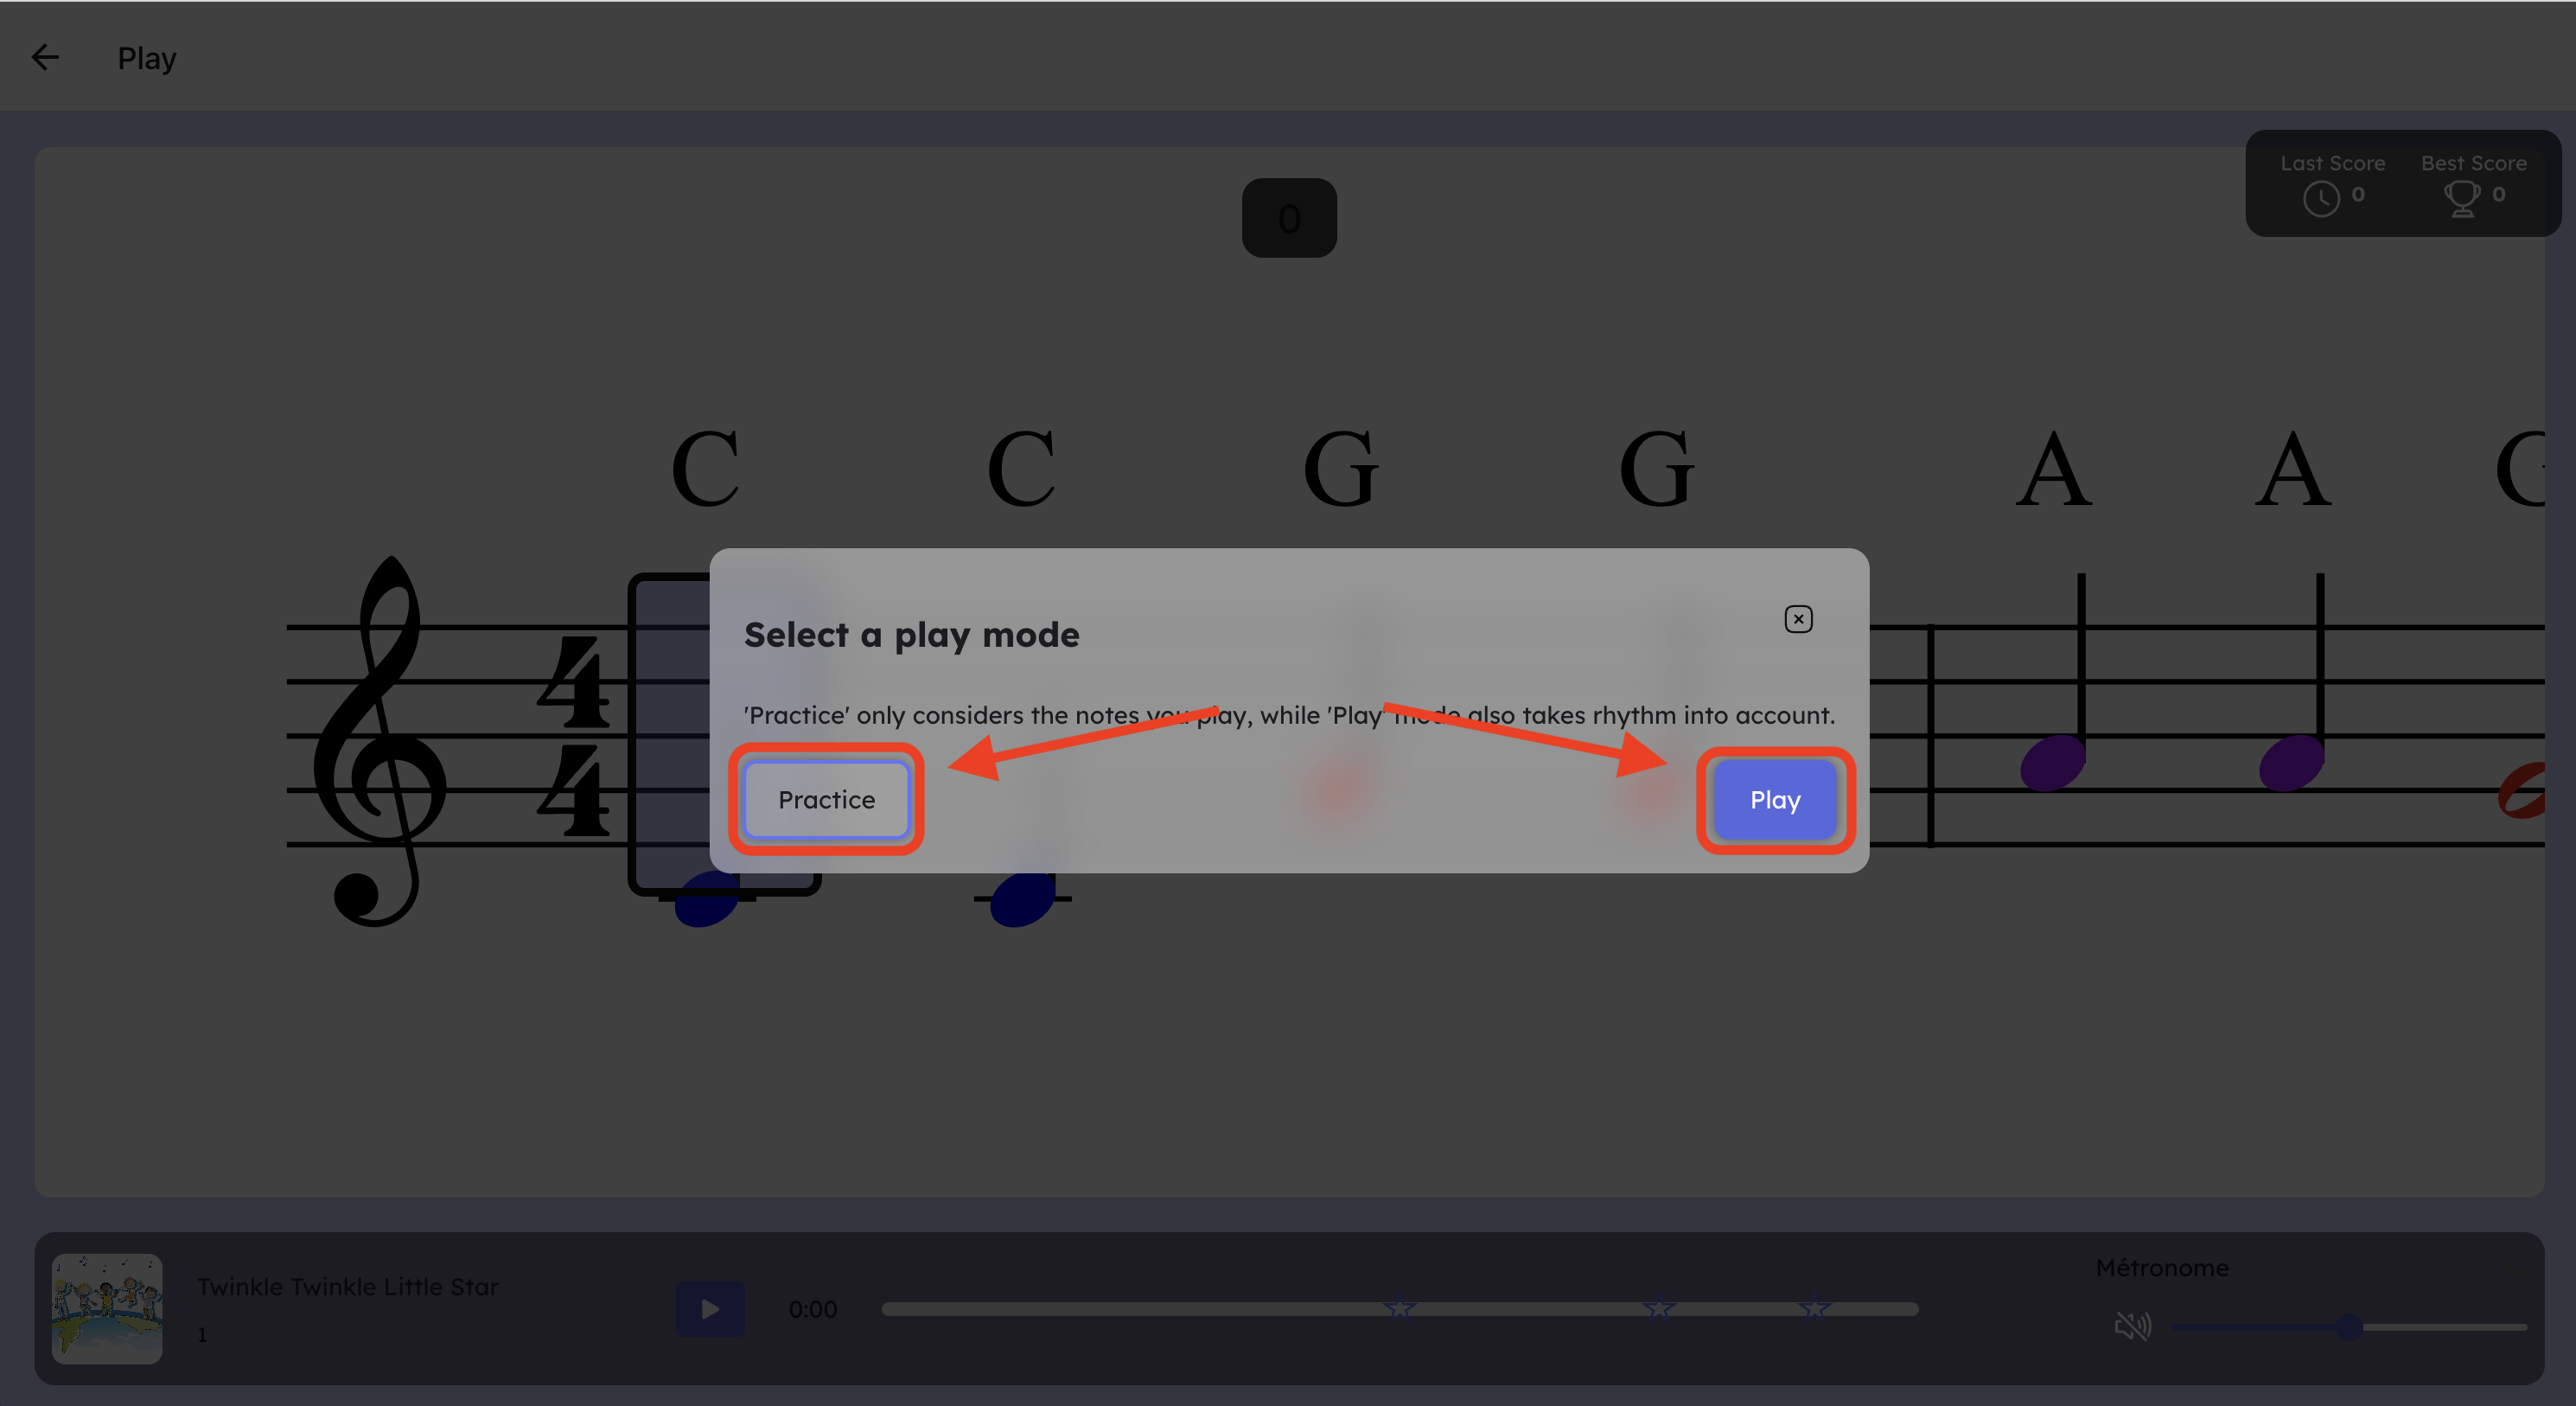
\includegraphics[width=\linewidth]{../\dir/guide/play/lobby.png}
	\caption{Lancer la partie depuis l'ecran de lobby}
\end{figure}

Vous arriverez sur la page de jeu. Pour lancer la partie, cliquez sur le bouton Play. Un compte à rebours de 3 secondes sera lancé. Lorsque celui-ci sera écoulé, la partie commencera, et la partition défilera.

\begin{figure}[H]
	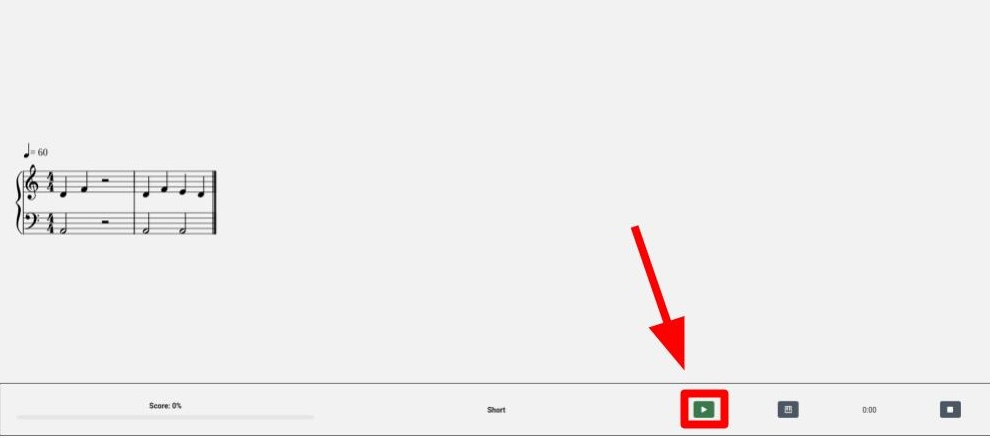
\includegraphics[width=\linewidth]{../\dir/guide/play/play.jpg}
	\caption{Lancer la partie}
\end{figure}

Vous pouvez faire pause à tout moment en cliquant sur le bouton pause. Vous pouvez stopper la partie en cliquant sur le bouton Stop.
\\\\
Une fois la partie terminée, vous serez redirigé vers votre page de score.

\begin{figure}[H]
	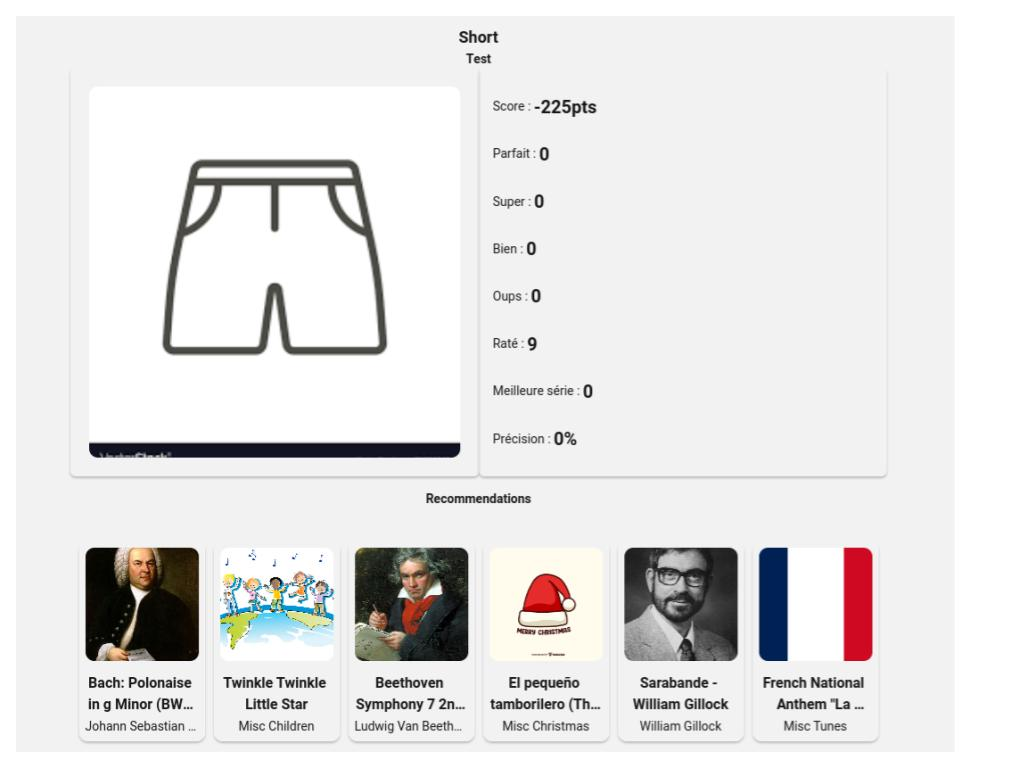
\includegraphics[width=\linewidth]{../\dir/guide/play/score.jpg}
	\caption{Score en fin de partie}
\end{figure}